\documentclass[aspectratio = 169, 13pt]{beamer}

% xcolor and define colors -------------------------
\usepackage{xcolor}

% https://www.viget.com/articles/color-contrast/
\definecolor{navy}{HTML}{567293}
\definecolor{purple}{HTML}{695693}
\definecolor{ruby}{HTML}{9a2515}
\definecolor{alice}{HTML}{107895}
\definecolor{daisy}{HTML}{EBC944}
\definecolor{coral}{HTML}{F26D21}
\definecolor{kelly}{HTML}{829356}
\definecolor{cranberry}{HTML}{E64173}
\definecolor{jet}{HTML}{131516}
\definecolor{asher}{HTML}{555F61}
\definecolor{slate}{HTML}{314F4F}

\newcommand\navy[1]{{\color{navy}#1}}
\newcommand\purple[1]{{\color{purple}#1}}
\newcommand\kelly[1]{{\color{kelly}#1}}
\newcommand\ruby[1]{{\color{ruby}#1}}
\newcommand\alice[1]{{\color{alice}#1}}
\newcommand\daisy[1]{{\color{daisy}#1}}
\newcommand\coral[1]{{\color{coral}#1}}
\newcommand\cranberry[1]{{\color{cranberry}#1}}
\newcommand\slate[1]{{\color{slate}#1}}
\newcommand\jet[1]{{\color{jet}#1}}
\newcommand\asher[1]{{\color{asher}#1}}

\newcommand\bgNavy[1]{{\colorbox{navy!80!white}{#1}}}
\newcommand\bgPurple[1]{{\colorbox{purple!80!white}{#1}}}
\newcommand\bgKelly[1]{{\colorbox{kelly!80!white}{#1}}}
\newcommand\bgRuby[1]{{\colorbox{ruby!80!white}{#1}}}
\newcommand\bgAlice[1]{{\colorbox{alice!80!white}{#1}}}
\newcommand\bgDaisy[1]{{\colorbox{daisy!80!white}{#1}}}
\newcommand\bgCoral[1]{{\colorbox{coral!80!white}{#1}}}
\newcommand\bgCranberry[1]{{\colorbox{cranberry!80!white}{#1}}}

% Mixtape Sessions
\definecolor{picton-blue}{HTML}{00b7ff}
\definecolor{violet-red}{HTML}{ff3881}
\definecolor{sun}{HTML}{ffaf18}
\definecolor{electric-violet}{HTML}{871EFF}

\newcommand\pictonBlue[1]{{\color{picton-blue}#1}}
\newcommand\sun[1]{{\color{sun}#1}}
\newcommand\electricViolet[1]{{\color{electric-violet}#1}}
\newcommand\violetRed[1]{{\color{violet-red}#1}}

\newcommand\bgPictonBlue[1]{{\colorbox{picton-blue!20!white}{#1}}}
\newcommand\bgSun[1]{{\colorbox{sun!20!white}{#1}}}
\newcommand\bgElectricViolet[1]{{\colorbox{electric-violet!20!white}{#1}}}
\newcommand\bgVioletRed[1]{{\colorbox{violet-red!20!white}{#1}}}

\def\code#1{\texttt{#1}}


% Main theme colors
\definecolor{accent}{HTML}{00b7ff}
\definecolor{accent2}{HTML}{871EFF}
\definecolor{gray100}{HTML}{f3f4f6}
\definecolor{gray800}{HTML}{1F292D}


% Beamer Options -------------------------------------

% Background
\setbeamercolor{background canvas}{bg = white}

% Change text margins
\setbeamersize{text margin left = 15pt, text margin right = 15pt} 

% \alert
\setbeamercolor{alerted text}{fg = accent2}

% Frame title
\setbeamercolor{frametitle}{bg = white, fg = jet}
\setbeamercolor{framesubtitle}{bg = white, fg = accent}
\setbeamerfont{framesubtitle}{size = \small, shape = \itshape}

% Block
\setbeamercolor{block title}{fg = white, bg = accent2}
\setbeamercolor{block body}{fg = gray800, bg = gray100}

% Title page
\setbeamercolor{title}{fg = gray800}
\setbeamercolor{subtitle}{fg = accent}

%% Custom \maketitle and \titlepage
%\setbeamertemplate{title page}
%{
%    %\begin{centering}
%        \vspace{20mm}
%        {\Large \usebeamerfont{title}\usebeamercolor[fg]{title}\inserttitle}\\
%        {\large \itshape \usebeamerfont{subtitle}\usebeamercolor[fg]{subtitle}\insertsubtitle}\\ \vspace{10mm}
%        {\insertauthor}\\
%        {\color{asher}\small{\insertdate}}\\
%    %\end{centering}
%}

% Table of Contents
\setbeamercolor{section in toc}{fg = accent!70!jet}
\setbeamercolor{subsection in toc}{fg = jet}

% Button 
\setbeamercolor{button}{bg = accent}

% Footnotes in Navigation Symbols
\setbeamertemplate{navigation symbols}{}

\usepackage{appendixnumberbeamer}
\setbeamercolor{page number in head/foot}{fg=alice}
\setbeamertemplate{footline}[frame number]


% Table and Figure captions
\setbeamercolor{caption}{fg=jet!70!white}
\setbeamercolor{caption name}{fg=jet}
\setbeamerfont{caption name}{shape = \itshape}

% Bullet points

%% Jon's itemize
\setbeamersize{text margin left=1em,text margin right=1em} 
\newenvironment{wideitemize}{\itemize\addtolength{\itemsep}{10pt}}{\enditemize}
\newenvironment{wideitemizeshort}{\itemize}{\enditemize}

%% Fix left-margins
\settowidth{\leftmargini}{\usebeamertemplate{itemize item}}
\addtolength{\leftmargini}{\labelsep}

%% enumerate item color
\setbeamercolor{enumerate item}{fg = accent}
\setbeamerfont{enumerate item}{size = \small}
\setbeamertemplate{enumerate item}{\insertenumlabel.}

\setbeamercolor{enumerate subitem}{fg = accent!60!white}
\setbeamerfont{enumerate subitem}{size = \small}
\setbeamertemplate{enumerate subitem}{\insertenumlabel.}

%% itemize
\setbeamercolor{itemize item}{fg = accent!70!white}
\setbeamerfont{itemize item}{size = \small}
\setbeamertemplate{itemize item}[circle]

%% right arrow for subitems
\setbeamercolor{itemize subitem}{fg = accent!60!white}
\setbeamerfont{itemize subitem}{size = \small}
\setbeamertemplate{itemize subitem}{$\rightarrow$}

\setbeamertemplate{itemize subsubitem}[square]
\setbeamercolor{itemize subsubitem}{fg = jet}
\setbeamerfont{itemize subsubitem}{size = \small}







% Links ----------------------------------------------

\usepackage{hyperref}
\hypersetup{
  colorlinks = true,
  linkcolor = accent2,
  filecolor = accent2,
  urlcolor = accent2,
  citecolor = accent2,
}


% Line spacing --------------------------------------
\usepackage{setspace}
\setstretch{1.2}


% \begin{columns} -----------------------------------
\usepackage{multicol}


% Fonts ---------------------------------------------
% Beamer Option to use custom fonts
\usefonttheme{professionalfonts}

% \usepackage[utopia, smallerops, varg]{newtxmath}
% \usepackage{utopia}
\usepackage[sfdefault,light]{roboto}

% Small adjustments to text kerning
\usepackage{microtype}



% Remove annoying over-full box warnings -----------
\vfuzz2pt 
\hfuzz2pt


% Table of Contents with Sections
\setbeamerfont{myTOC}{series=\bfseries, size=\Large}
\AtBeginSection[]{
        \frame{
            \frametitle{Roadmap}
            \tableofcontents[current]   
        }
    }


% Tables -------------------------------------------
% Tables too big
% \begin{adjustbox}{width = 1.2\textwidth, center}
\usepackage{adjustbox}
\usepackage{array}
\usepackage{threeparttable, booktabs, adjustbox}
    
% Fix \input with tables
% \input fails when \\ is at end of external .tex file
\makeatletter
\let\input\@@input
\makeatother

% Tables too narrow
% \begin{tabularx}{\linewidth}{cols}
% col-types: X - center, L - left, R -right
% Relative scale: >{\hsize=.8\hsize}X/L/R
\usepackage{tabularx}
\newcolumntype{L}{>{\raggedright\arraybackslash}X}
\newcolumntype{R}{>{\raggedleft\arraybackslash}X}
\newcolumntype{C}{>{\centering\arraybackslash}X}

% Figures

% \imageframe{img_name} -----------------------------
% from https://github.com/mattjetwell/cousteau
\newcommand{\imageframe}[1]{%
    \begin{frame}[plain]
        \begin{tikzpicture}[remember picture, overlay]
            \node[at = (current page.center), xshift = 0cm] (cover) {%
                \includegraphics[keepaspectratio, width=\paperwidth, height=\paperheight]{#1}
            };
        \end{tikzpicture}
    \end{frame}%
}

% subfigures
\usepackage{subfigure}


% Highlight slide -----------------------------------
% \begin{transitionframe} Text \end{transitionframe}
% from paulgp's beamer tips
\newenvironment{transitionframe}{
    \setbeamercolor{background canvas}{bg=accent!40!black}
    \begin{frame}\color{accent!10!white}\LARGE\centering
}{
    \end{frame}
}


% Table Highlighting --------------------------------
% Create top-left and bottom-right markets in tabular cells with a unique matching id and these commands will outline those cells
\usepackage[beamer,customcolors]{hf-tikz}
\usetikzlibrary{calc}
\usetikzlibrary{fit,shapes.misc}

% To set the hypothesis highlighting boxes red.
\newcommand\marktopleft[1]{%
    \tikz[overlay,remember picture] 
        \node (marker-#1-a) at (0,1.5ex) {};%
}
\newcommand\markbottomright[1]{%
    \tikz[overlay,remember picture] 
        \node (marker-#1-b) at (0,0) {};%
    \tikz[accent!80!jet, ultra thick, overlay, remember picture, inner sep=4pt]
        \node[draw, rectangle, fit=(marker-#1-a.center) (marker-#1-b.center)] {};%
}



% References ----------------------------------------

%% Bibliography Font, roughly matching aea
\setbeamerfont{bibliography item}{size = \footnotesize}
\setbeamerfont{bibliography entry author}{size = \footnotesize, series = \bfseries}
\setbeamerfont{bibliography entry title}{size = \footnotesize}
\setbeamerfont{bibliography entry location}{size = \footnotesize, shape = \itshape}
\setbeamerfont{bibliography entry note}{size = \footnotesize}

\setbeamercolor{bibliography item}{fg = jet}
\setbeamercolor{bibliography entry author}{fg = accent!60!jet}
\setbeamercolor{bibliography entry title}{fg = jet}
\setbeamercolor{bibliography entry location}{fg = jet}
\setbeamercolor{bibliography entry note}{fg = jet}

%% Remove bibliography symbol in slides
\setbeamertemplate{bibliography item}{}


% Citations ----------------------------------------
\usepackage{natbib}
%\bibliographystyle{apalike}
\bibliographystyle{aer}

\usepackage{bibunits}
\defaultbibliography{Bibliography.bib}  
%\defaultbibliographystyle{apalike}
\defaultbibliographystyle{aer}

\newcommand{\backupbegin}{
  \newcounter{finalframe}
  \setcounter{finalframe}{\value{framenumber}}
}
\newcommand{\backupend}{
  \setcounter{framenumber}{\value{finalframe}}
}

\input{preambles/notation.tex}
\author{Jonathan Roth}
\title[Pre-trends testing]{Testing and Sensitivity Analysis for Violations of Parallel Trends}

\begin{document}

%\imageframe{figures/cover_violations.png}
\maketitle	


\begin{frame}{Outline}
	\begin{wideitemize}
		\item
		What is the parallel trends assumption? 
		
		\item
		Why might we be initally skeptical of the parallel trends assumption? 
		
		\item
		How can we partially test the validity of parallel trends using pre-treatment info? 
		
		\item
		Limitations of pre-trends tests
		
		\item
		Alternative approaches when worried about violations of parallel trends
	\end{wideitemize}
\end{frame}

\begin{frame}{Set-up}
For simplicity, consider the canonical two-period DiD model:
\medskip
\begin{wideitemize}
	\item
	There are two periods, $t=0,1$
	
	\item
	We observe panel data with outcomes $Y_{it}$ for individual $i$ in period $t$
	
	\item
	Units with $D_i=1$ are treated beginning period 1; units with $D_i=0$ are never treated
	
	\item
	Potential outcomes: observed outcome is $Y_{it} = D_i Y_{it}(1) + (1-D_i) Y_{it}(0)$
	
	\item
	Assume ``no anticipation'': $Y_{i0}(0) = Y_{i0}(1)$
\end{wideitemize}
\end{frame}

\begin{frame}{What is parallel trends?}
	\begin{wideitemize}
		\item
		The \textbf{parallel trends} assumption states that if the treatment hadn't occurred, average outcomes for the treatment and control groups would have evolved in parallel
		
		$$\underbrace{ E[Y_{i1}(0) - Y_{i0}(0) \mid D_i =1] }_{\text{Counterfactual change for treated group}}= \underbrace{ E[Y_{i1}(0) - Y_{i0}(0) \mid D_i =0] }_{\text{Change for untreated group}} $$ 
		
		\pause
		\item
		The parallel trends assumption can also be viewed as a \textbf{selection bias stability} assumption:  
		$$\underbrace{ E[Y_{i1}(0)  \mid D_i =1] - E[Y_{i1}(0) \mid D_i=0] }_{\text{Selection bias in period 1}}= \underbrace{ E[Y_{i0}(0)  \mid D_i =1] - E[Y_{i0}(0) \mid D_i=0] }_{\text{Selection bias in period 0}} $$ 
		
		\pause
		\item
		PT allows for there to be selection bias!\\
		However, the selection bias has to be the same in both periods
		
	\end{wideitemize}
\end{frame}

\begin{frame}{Visualizing PT}
	\begin{tikzpicture}[scale = 1.5]
		% Draw x-axis
		\draw[->] (0,0) -- (2.5,0) node[right] {Time};
		\draw (0,-0.1) -- (0,0.1);
		\draw (2,-0.1) -- (2,0.1);
		\node[below] at (0,-0.1) {0};
		\node[below] at (2,-0.1) {1};
		
		% Draw red dotted line
		\draw[red,dotted] (0,2) -- (2,2.5) node[above] {$E[Y(0) | Treated]$};
		
		% Draw blue solid line
		\draw[blue] (0,0.5) -- (2,1) node[midway,below=10pt] {$E[Y(0) | Control]$};
		
		% Add curly brace
		\draw[decorate,decoration={brace,amplitude=10pt}] (-0.2,0.5) -- (-0.2,2) node[midway,left=12pt] {Selection bias in period 0};
		
		% Add curly brace
		\draw[decorate,decoration={brace,amplitude=10pt,mirror}] (2.2,1) -- (2.2,2.5) node[midway,right=12pt] {Selection bias in period 1};
		
	\end{tikzpicture}
\end{frame}


\begin{frame}{Why is PT Useful? It allows us to identify the ATT!}

\medskip	

\begin{minipage}{0.4\linewidth}
			\begin{tikzpicture}[scale = 1.5]
		% Draw x-axis
		\draw[->] (0,0) -- (2.5,0) node[right] {Time};
		\draw (0,-0.1) -- (0,0.1);
		\draw (2,-0.1) -- (2,0.1);
		\node[below] at (0,-0.1) {0};
		\node[below] at (2,-0.1) {1};
		
		% Draw red dotted line
		\draw[red,dotted] (0,2) -- (2,2.5);
		
		\node[below,red] at (1.5,2) {$E[Y(0) | Treated]$};
		
		% Draw red dotted line
		\draw[red] (0,2) -- (2,3.5) node[above] {$E[Y | Treated]$};
		
		% Draw blue solid line
		\draw[blue] (0,0.5) -- (2,1) node[midway,below=10pt] {$E[Y | Control]$};
		
		% Add curly brace
		\draw[decorate,decoration={brace,amplitude=10pt,mirror}] (2.2,2.5) -- (2.2,3.5) node[midway,right=12pt] {ATT};			
	\end{tikzpicture}			
\end{minipage}%
\begin{minipage}{0.6\linewidth}
$$\underbrace{E[Y_{i1}(1)- Y_{i1}(0) | D_i =1]}_{ATT} = (\mu_{11} - \mu_{10}) - (\mu_{01} - \mu_{00})  $$
\noindent for $\mu_{td} = E[Y_{it} | D_i = 1]$.
\end{minipage}		
	

\end{frame}



\begin{frame}{Why might we be skeptical of PT?}
	\begin{wideitemize}
		\item
		Recall PT requires the selection bias to be constant over time.\\
		Why might we be skeptical of this? 
		
		\pause
		\item
		There might be different confounding factors in period 1 as in period 0 
			\begin{itemize}
				\item
				E.g. states that pass a minimum wage increase might also change unemployment insurance at the same time
				
				\item
				Then UI is a confound in period 1 but not in period 0
			\end{itemize}
		
		\pause
		\item
		The same confounding factors may have different effects on the outcome in different time periods
			\begin{itemize}
				\item
				Suppose people who enroll in a job training program are more motivated to find a job
				
				\item
				Motivation might matter more in a bad economy than in a good economy
			\end{itemize}
	\end{wideitemize}
\end{frame}


\begin{frame}{Why might we be skeptical of PT? Part 2}
	\begin{wideitemize}
		\item
		Another reason to be skeptical of parallel trends is that its validity will often be \textbf{functional form} dependent
		
		\item
		Consider an example: 
		\begin{wideitemize}
			\item 
			In period 0, all control units have outcome 10;  all treated units have outcome 5.
			
			\item
			In period 1, all control units have outcome 15.
			
			\item
			If treatment hadn't occurred, would treated units' outcome have increased by 5 also (PT in levels)? 
			
			\item
			Or would they have increased by 50\% ($\sim$ PT in logs)?
			
		\end{wideitemize} 

	\end{wideitemize}
\end{frame}

\begin{frame}{}
	
	\citet{roth_when_2023} show that PT will depend on functional form unless: \medskip 
	\begin{wideitemize}
		\item
		\textbf{Randomization:} treated and control group have same dist. of $Y(0)$ in each period
		
		\item
		\textbf{No time effects:} distribution of $Y(0)$ doesn't change over time for either group
		
		\item
		\textbf{A hybrid}: $\theta$ fraction of the population is as good as randomized; the other $1-\theta$ fraction has no time effects. 
	\end{wideitemize}
\bigskip 
Absent these conditions, PT will be violated for at least some functional form; often hard to know if we chose the right one!
\end{frame}


\begin{frame}{Pre-trends to the rescue...}
	\begin{wideitemize}
		\item
		Luckily, in most DiD applications we have several periods before anyone was treated
		
		\item
		We can test whether the groups were moving in parallel prior to the treatment
			\begin{wideitemize}
				\item
				If so, then assumption that confounding factors are stable seems more plausible
				
				\item
				If not, then it's relatively implausible that would have magically started moving in parallel after treatment date
			\end{wideitemize}
		
		\item
		Testing for pre-trends provides a natural plausibility check on the parallel trends assumption
	\end{wideitemize}
\end{frame}

\begin{frame}
	\begin{minipage}{.5\linewidth}
			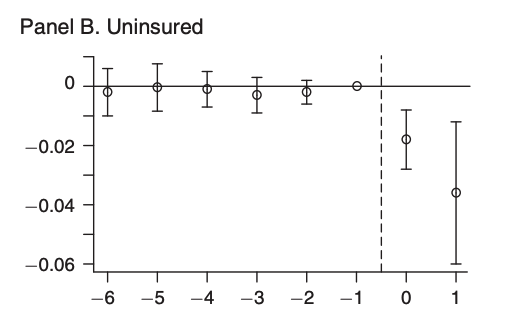
\includegraphics[width=0.99\linewidth]{Figures/Carey-event-study.png}
	\end{minipage}%
\begin{minipage}{0.5\linewidth}
	\begin{wideitemize}
	\item
	Carey, Miller, and Wherry (2020) do a DiD comparing states who expanded Medicaid in 2014 to states that didn't. 
	
	\item
	Report results from ``event-study'' regression: 
	$$Y_{its} =  \phi_{t} + \lambda_s + \sum_{r\neq -1}  D_i \times 1[t = 2014 + r] \cdot  \beta_r   + \epsilon_{it} $$
	
	\noindent where $Y_{its}$ is insurance for person $i$ in year $t$ in state $s$, and $D_i = 1$ if in an expansion state.
\end{wideitemize}
\end{minipage}


\end{frame}

\begin{frame}
	
	\begin{wideitemize}
		
	\item
	Testing for pre-existing trends is a very natural way to assess the plausibility of the PT assumption
	
	\item
	But it also has several \textit{limitations}, highlighted in recent work \citep[][]{freyaldenhoven_pre-event_2019, kahn-lang_promise_2020, bilinski_seeking_2018, roth_pre-test_2021}
	
	\item
	Remainder of the talk today will focus on these issues, as well as some solutions. 
	
	\item
	Perhaps selfishly, will focus mainly on two of my papers
	
	\begin{wideitemize}
		\item
		Roth (2022 AER:I, ``Pre-test with Caution: Event-study Estimates After Testing for Parallel Trends") 
		\item
		Rambachan and Roth (Forthcoming RESTUD, ``A More Credible Approach to Parallel Trends'') 
	\end{wideitemize}
	
	
	\end{wideitemize}

	
\end{frame}


\begin{frame}{Overview of Limitations}
	\begin{wideitemize}
		\item
		Parallel pre-trends doesn't necessarily imply parallel (counterfactual) post-treatment trends
			\begin{wideitemize}
				\item
				If other policies change at the same time as the one of interest --- e.g. min wage and UI reform together --- can produce parallel pre-trends but non-parallel post-trends
				
				\item
				Likewise, could be that treated/control groups are differentially exposed to recessions, but there is only a recession in the post-treatment period
			\end{wideitemize}
		
		\pause
		\item
		\textbf{Low power:} even if pre-trends are non-zero, we may fail to detect it statistically
		
		\pause
		\item
		\textbf{Pre-testing issues:} if we only analyze cases without statistically significant pre-trends, this introduces a form of selection bias (which can make things worse) 
		
		\pause
		\item
		If we fail the pre-test, what next? May still want to write a paper (especially if violation is ``small'')
	\end{wideitemize}
\end{frame}



\begin{frame}{Issue 1 - Low Power}
  \begin{center}
		\includegraphics<1>[width = .6\textwidth]{figures/HeAndWangAnimations/HeAndWang-base.png}
  \end{center}
	
	\begin{itemize}
		\item 
    He \& Wang (2017) study impacts of placing college grads as village officials in China
		          
		\item
    Use an ``event-study'' approach comparing treated and untreated villages
    \vspace{-2mm}
    $$
    Y_{it} = \sum_{k \neq -1} D_{it}^k \beta_k + \alpha_i + \phi_t + \epsilon_{it}
    $$
	\end{itemize}
\end{frame}

\begin{frame}{Issue 1 - Low Power}
  \begin{center}
		\includegraphics<1>[width = .6\textwidth]{figures/HeAndWangAnimations/HeAndWang-base.png}   
		\includegraphics<2>[width = .6\textwidth]{figures/HeAndWangAnimations/HeAndWang-ZeroDots.png} 
		\includegraphics<3>[width = .6\textwidth]{figures/HeAndWangAnimations/HeAndWang-RedDots.png} 
		\includegraphics<4>[width = .6\textwidth]{figures/HeAndWangAnimations/HeAndWang-RedTrend.png} 
		\includegraphics<5>[width = .6\textwidth]{figures/HeAndWangAnimations/HeAndWang-BlueDots.png}
		\includegraphics<6->[width = .6\textwidth]{figures/HeAndWangAnimations/HeAndWang-BlueTrend.png}
  \end{center}  
	
	\begin{onlyenv}<1>
		\begin{quote}
			``The estimated coefficients on the leads of treatment ... are \textit{statistically indifferent from 0}. ... We conclude that \textit{the pretreatment trends in the outcomes in both groups of villages are similar}, and villages without CGVOs \textit{can serve as a suitable control group} for villages with CGVOs in the treatment period.'' (He and Wang, 2017)
			    
		\end{quote}
	\end{onlyenv}
	{\footnotesize
	\begin{itemize}
		\item<2-> P-value for $H_0: \betapre = $ {\color{green} green dots} (no pre-trend): 0.81
		\item<3-> P-value for $H_0: \betapre = $ {\color{red} red dots}: 0.81
		\item<5-> P-value for $H_0: \betapre = $ {\color{blue} blue dots}: 0.81
		    
		\item<7-> We can't reject zero pre-trend, but we also can't reject pre-trends that under smooth extrapolations to the post-treatment period would produce substantial bias
	\end{itemize}
  }
	
\end{frame}



\begin{frame}[label = roth sims]{More systematic evidence}
	
	\begin{wideitemize}
		
		\item
		Roth (2022): simulations calibrated to papers published in \textit{AER}, \textit{AEJ: Applied}, and \textit{AEJ: Policy} between 2014 and mid-2018  
		\begin{itemize}
			\item
			      70 total papers contain an event-study plot; focus on 12 w/available data
		\end{itemize}
		
		\item
		Evaluate properties of standard estimates/CIs under linear violations of parallel trends against which conventional tests have limited power (50 or 80\%):
		
		\begin{enumerate}
			\normalsize{
				\item
				Bias often of magnitude similar to estimated treatment effect
				    
				\item
				Confidence intervals substantially undercover in many cases
				    
				\item
				Distortions from pre-testing can further exacerbate these issues
			}
		\end{enumerate}
	\end{wideitemize}
	
\end{frame}

\begin{frame}{Issue 2 - Distortions from Pre-testing}
	\begin{wideitemize}
		\item
		When parallel trends is violated, we will sometimes fail to find a significant pre-trend
		
		\item
		But the draws of data where this happens are a \textbf{selected sample}. This is known as \textit{pre-test bias}.
		
		\item
		Analyzing this selected sample introduces additional statistical issues, and can make things worse!
		
	\end{wideitemize}
\end{frame}

\begin{frame}{Stylized Three-Period DiD Example}
	
	\begin{itemize}
		\item 
    Consider a 3-period model ($t=-1,0,1$) where treatment occurs in last period
		      
		          
    \bigskip
		\item
    No causal effect of treatment: $Y_{it}(0) = Y_{it}(1)$ in all periods
		          
    \bigskip
		\item
    In population, treatment group is on a linear trend relative to the control group with slope $\delta$
    \medskip
    \begin{itemize}
      {\normalsize
        \item
        Control group mean in period $t$: $E[ Y_{it}(0) \mid \text{Control group} ] = 0 $
		      		            
        \item
        Treatment group mean in period $t$: $E[ Y_{it}(0) \mid \text{Treated group} ] = \delta \cdot t$
      }
    \end{itemize}
	\medskip		          
  
			\item
		Simulate from this model with $Y_{it}$ equal to the group mean plus independent normal errors
      
		      
	\end{itemize}
\end{frame}


\begin{frame}
	\centering
	\includegraphics<1>[width = .8\columnwidth]{figures/IntuitionPlots/PopulationMeans.png}
	
	\includegraphics<2>[width = .8\columnwidth]{figures/IntuitionPlots/DataDraws_Unhighlighted.png}
	
	\includegraphics<3-4>[width = .8\columnwidth]{figures/IntuitionPlots/DataDraws_Highlighted.png}
	
	\includegraphics<5>[width = .8\columnwidth]{figures/IntuitionPlots/PopulationMeans_PopulationAndInsignificant_Annotated.png}
	
	
	% \includegraphics<6>[width = \columnwidth]{figures/IntuitionPlots/DistributionDeltaY0_PopulationAndInsiginificant.png}
	
	
	% \includegraphics<6>[width = \columnwidth]{figures/IntuitionPlots/Distributions_PopulationAndInsiginificant.png}
	
	
	
	\begin{itemize}
		
		\begin{onlyenv}<1-3>
			\item
			Example: In population, there is a linear difference in trend with slope 3    
		\end{onlyenv}
		
		\begin{onlyenv}<2>
			\item
			In actual draws of data, there will be noise around this line
		\end{onlyenv}
		
		\begin{onlyenv}<3-4>
			\item
			In some of the draws of the data, highlighted in blue, the difference between period -1 and 0 will be insignificant
		\end{onlyenv}
		
		\begin{onlyenv}<4-5>
			\item
			In the insignificant draws, we tend to underestimate the difference between treatment and control at $t=0$
		\end{onlyenv}
		
		\begin{onlyenv}<5>
			\item
			As a result, the DiD between period 0 and 1 tends to be particularly large when we get an insignificant pre-trend
		\end{onlyenv}
	\end{itemize}
	
\end{frame}



\begin{frame}{To Summarize}
	
	\textbf{What are the Statistical Limitations of Pre-trends Testing?}
	\begin{enumerate}
		\item
		      Low Power -- May not find significant pre-trend even if PT is violated
		          
		\item
		      Pre-testing Issues -- Selection bias from only analyzing cases with insignificant pre-trend
		          
		\item
		      If reject pre-trends test, what comes next? 
	\end{enumerate}
	
	\bigskip
	\pause 
	
	\textbf{What Can We Do About It?}
	\begin{enumerate}
		\item 
		      Diagnostics of power and distortions from pre-testing (Roth, 2022, ``Pre-Test with Caution..."). See \texttt{pretrends} package. \hyperlink{power_analysis}{\beamerbutton{Details}}
		          
		\item
		      Formal sensitivity analysis that avoids pre-testing (Rambachan and Roth, Forthcoming, ``A More Credible Approach...''). See \texttt{HonestDiD} package.
		          
	\end{enumerate}
	
\end{frame}




\begin{frame}{``A More Credible Approach to Parallel Trends''}
	\begin{wideitemize}
		
		
		\item The intuition motivating pre-trends testing is that the pre-trends are informative about counterfactual post-treatment trends
		
		\item Formalize this by imposing the restriction that the counterfactual difference in trends can't be ``too different'' than the pre-trend
		
		
		\item This allows us to bound the treatment effect and obtain uniformly valid (``honest'') confidence sets under the imposed restrictions
		    
		    
		\item Enables \textbf{sensitivity analysis:} How different would the counterfactual trend have to be from the pre-trends to negate a conclusion (e.g. a positive effect)?
		    
	\end{wideitemize}
	
\end{frame}

\begin{frame}{Restrictions on Violations of PT}
	\begin{wideitemize}
		
		\item
		Consider the 3-period model ($t=-1,0,1$) where treatment occurs in last period
		
		\item
		Let $\delta_1$ be the violation of PT:
		
		$$\delta_1 = \expe{ Y_{i,t=1}(0) - Y_{i,t=0}(0) \,|\, D_i = 1} - \expe{ Y_{i,t=1}(0) - Y_{i,t=0}(0) \,|\, D_i = 0} $$
		
		\item
		We don't directly identify $\delta_1$, but we do identify its pre-treatment analog, $\delta_{-1}$:
		
		$$\delta_{-1} = \expe{ Y_{i,t=-1}(0) - Y_{i,t=0}(0) \,|\, D_i = 1} - \expe{ Y_{i,t=-1}(0) - Y_{i,t=0}(0) \,|\, D_i = 0} $$
		
		\item
		Key idea: restrict possible values of $\delta_1$ given $\delta_{-1}$ \\
		
		Intuitively, counterfactual trend can't be too different from pre-trend
		
	\end{wideitemize}
\end{frame}


\begin{frame}{Examples of Restrictions on $\delta$}
	\begin{wideitemize}
		
		\item \textbf{Bounds on relative magnitudes:} Require that $|\delta_1| \leq \bar{M} |\delta_{-1}|$
		
		\pause
		
		\item \textbf{Smoothness restriction:} Bound how far $\delta_1$ can deviate from a linear extrapolation of the pre-trend: $\delta_1 \in [-\delta_{-1}-M , -\delta_{1} + M]$
		
	\end{wideitemize}
	
	\centering
	\includegraphics[width = 0.7\textwidth]{figures/IntuitionPlots/Delta-Examples/deltaSD.png}
	
\end{frame}


\begin{frame}{Robust confidence intervals}
	\begin{wideitemize}
		\item
		In the paper, we develop confidence intervals for the treatment effect of interest under the assumptions on $\delta$ discussed above
		
		\item
		The CIs account for the fact that we don't observe the true (population) pre-trend $\deltapre$, only our estimate $\betahatpre$. 
		
		\item
		The robust CIs tend to be wider the larger are the confidence intervals on the pre-trends --- intuitive, since if we know less about the pre-trends, we should have more uncertainty
		
		\item
		This contrasts with pre-trends tests, where you're less likely to reject the null that $\betapre =0$ when the SEs are larger!
	\end{wideitemize}
\end{frame}


\begin{frame}{Benzarti \& Carloni (2019)}
	\begin{wideitemize}
		\item
		BC study the incidence of a cut in the value-added tax on sit-down restaurants in France.
		France reduced the VAT on restaurants from 19.6 to 5.5 percent in July of 2009. 
		
		\item
		BC analyze the impact of this change using a difference-in-differences design comparing restaurants to a control group of other market services firms
		\vspace{-3mm}
		\begin{equation}
			Y_{irt} = \sum_{s = 2004}^{2012} \beta_s \times 1[t = s] \times  D_{ir} + \phi_i + \lambda_t + \epsilon_{irt} , \label{eqn: bc event-study spec}    
		\end{equation}
		\vspace{-3mm}
		\noindent 
    \begin{itemize}
      \item $Y_{irt}$ = outcome of interest for firm $i$ in region $r$
      \item $D_{ir}$ = indicator if firm $i$ in region $r$ is a restaurant
      \item $\Phi_i, \lambda_t$ = firm and year FEs
		\end{itemize}
		
		\item Outcomes of interest include firm profits, prices, wage bill \& employment.\\
		We focus on impact on profits in first year after reform.
	\end{wideitemize}
\end{frame}


\begin{frame}{Event-study coefficients for log profits}
	\centering
	\includegraphics[width = 0.8 \textwidth]{figures/Benzarti-Carloni/profits-event-study.png}
\end{frame}

\begin{frame}
	{\centering
		\includegraphics[width = 0.4\linewidth]{figures/Benzarti-Carloni/sensitivity-MB-profits.png}
	}
	
	\begin{itemize}
		\item
		      ``Breakdown'' $\bar{M}$ for null effect using relative magnitudes bounds is $\sim 2$
		          
		\item
		      Can rule out a null effect unless allow for violations of PT 2x larger than the max in pre-period
		      
	\end{itemize}
	
\end{frame}

\begin{frame}{Extension to other estimators}
	\begin{wideitemize}
		\item
		So far we focused on sensitivity analysis for ``simple'' event-studies
		
		\item
		However, the key idea was that we were willing to restrict the bias of some post-treatment event-study estimates $\betahatpost$ using the expectation of some pre-treatment event-study estimates $\betahatpre$
		
		\item
		This idea extends to any asymptotically normal event-study estimates $(\betahatpre, \betahatpost)$!
		
		\item
		This includes:
		
		\begin{itemize}
			\item
			Event-studies for settings with staggered treatment timing \citep[e.g.][]{callaway_difference--differences_2020, sun_estimating_2020}
			
			\item
			IV event-studies \citep[][]{hudson_interpreting_2017}
			
			\item
			Flexible methods for controlling for covariates \citep{santanna_doubly_2020}
		\end{itemize}
	\end{wideitemize}
\end{frame}



\begin{frame}{So to summarize!}
	\begin{wideitemize}
		\item
		Tests of pre-trends are intuitive but not a panacea!
		    
		\item
		In particular, they may suffer from low power and introduce pre-test bias
		    
		\item
		Roth (2022) and Rambachan and Roth (Forthcoming) provide tools for diagnostics and sensitivity analysis
		    
		\item
		And these tools play nicely with recent estimators developed for heterogeneous treatment effects; see the bonus question in the coding exercise for an example!
		    
	\end{wideitemize}
\end{frame}

\begin{frame}{Other Related Papers}
	
	\begin{wideitemize}
		
		\item
		Other bounding exercises \citep{manski_how_2017, ye_negative_2021}
		
		\item
		Non-inferiority approaches to pre-testing \citep{bilinski_no_2018, dette_difference--differences_2020}
		
		\item
		Impose structure on the confounds \citep{freyaldenhoven_pre-event_2019}
	\end{wideitemize}
	    
\end{frame}


% \begin{frame}{Wrapping Up}

% \begin{wideitemize}

% \item
% Tests of pre-trends are intuitive but not a panacea!

% \item
% Roth (2021) and Rambachan and Roth (2021) provide tools for diagnostics and sensitivity analysis

% \item
% It's important to incorporate \textit{context-specific} knowledge when using these tools.

% \item
% \textbf{Think about how parallel trends may be violated in your context!}\\
% This puts the ``econ'' back into ``econometrics''
% \end{wideitemize}
    
% \end{frame}



\appendix


\begin{frame}[noframenumbering,plain]
	\centering
	Thank you!
\end{frame}


\begin{frame}{Additional Resources}
	\begin{wideitemize}
		\item
		Roth (2022 AER:I, ``Pre-test with Caution: Event-study Estimates After Testing for Parallel Trends''
		\begin{itemize}
			\item 
			      \href{https://jonathandroth.github.io/assets/files/roth_pretrends_testing.pdf}{Paper}; \href{https://github.com/jonathandroth/pretrends}{\texttt{staggered} package} ; \href{https://github.com/jonathandroth/PretrendsPower\#pretrendspower}{Shiny app}
		\end{itemize}
		    
		\item
		Rambachan and Roth (2023 RESTUD), ``A More Credible Approach to Parallel Trends'''
		\begin{itemize}
			\item 
			      \href{https://jonathandroth.github.io/assets/files/HonestParallelTrends_Main.pdf}{Paper}; \href{https://github.com/asheshrambachan/HonestDiD}{\texttt{HonestDiD} package} ; \href{https://github.com/asheshrambachan/HonestDiD/blob/master/doc/HonestDiD_Example.pdf}{Vignette}
		\end{itemize}
	\end{wideitemize}
\end{frame}

\begin{frame}[label = power_analysis]{Pre-testing Diagnostics}
	\begin{wideitemize}
		\item
		A ``low-touch'' intervention is to evaluate the likely power/distortions from pre-testing under \textit{context-relevant} violations of parallel trends
		
		\item Enter the \texttt{pretrends} package / Shiny app
	\end{wideitemize}
\end{frame}

\begin{frame}
	\centering
	\includegraphics[height = 0.9 \textheight]{figures/Shiny-Mockup-Graph-Only.png}   
\end{frame}

\begin{frame}
	\centering
	\includegraphics[width = 0.7 \textwidth]{figures/Shiny-Mockup-Power-Only.png} 
	\begin{wideitemize}
		\item
		\textbf{Power.} Chance find significant pre-trend under hypothesized trend.
		\item
		\textbf{Bayes Factor.} Relative chance you pass the pre-test under hypothesized trend versus under parallel trends.
		\item
		\textbf{Likelihood Ratio.} Likelihood of observed pre-trend coefs under hypothesized trend versus under parallel trends.
	\end{wideitemize}
\end{frame}

\begin{frame}{Pros and Cons}
	\textbf{Pros}
	\begin{wideitemize}
		\item
		Very intuitive, easy to visualize.
		
		\item
		Helps identify when pre-testing may be least effective
		    
		\item
		Requires minimal changes from standard practice
	\end{wideitemize}
	
	\textbf{Cons}
	
	\begin{wideitemize}
		\item
		Power will always be $<1$, so no guarantee of unbiasedness/correct inference
		    
		\item
		Need to specify the hypothesized trend. Will sometimes be difficult to summarize over many of these.
		    
		\item
		Still not clear what to do when reject the pre-test.
	\end{wideitemize}
	    
\end{frame}

\begin{frame}[allowframebreaks,noframenumbering,plain]{References}
	\nocite{rambachan_honest_2021}
	\bibliography{Bibliography.bib}
\end{frame}


\end{document} 
